\samepage{
\chapter{Results}\label{chapter:results}

In this chapter I present how my CUDA solution compares against the TensorFlow Implementations of $\Phi_{Flow}$.
\par All benchmarks were performed in a closed boundary environment with random divergence vectors in the $\left[-1, 1 \right]$ range. The targeted residual accuracy was $1^{-5}$. Before starting the measurement, a warm-up of 5 runs was performed. The data show the mean and standard deviation of 25 runs. The test system consists of a GeForce GTX 980, a Quad-Core Intel Core i7 3779K @3.5GHz CPU and 8GB of RAM.
\subsubsection{Performance Pressure Solve}
The following table shows the execution time for quadratic grids and compares the Tensorflow solutions with my CUDA implementation: \\\\
\renewcommand{\arraystretch}{1.39}
\begin{tabular}{c|l|l|l|c|c}
\hline
Dimension& TF CPU   & TF GPU   & CUDA     & Speedup TF CPU & Speedup TF GPU \\ \hline
$16^2$   & 8,293 ms & 28,30 ms & 9,391 ms & 0.9 x   & 3.0 x  \\ \hline
$32^2$   & 17,27 ms & 48,76 ms & 14,65 ms & 1.2 x   & 3.3 x  \\ \hline
$64^2$   & 49,65 ms & 108,2 ms & 25,36 ms & 2.0 x   & 4.2 x  \\ \hline
$128^2$  & 207,6 ms & 396,3 ms & 39,49 ms & 5.3 x   & 10.0 x \\ \hline
$256^2$  & 1,169 s  & 1,839 s  & 77,19 ms & 15.1 x  & 23.8 x \\ \hline
$512^2$  & 12,75 s  & 12,90 s  & 240,9 ms & 52.9 x  & 53.6 x \\ \hline
$1024^2$ & 133.7 s  & 87,47 s  & 1,412 s  & 94.6 x  & 61.9 x \\ \hline
$2048^2$ & n/a      & n/a      & 9,742 s  & n/a     & n/a    \\ \hline \hline

$16^3$   & 40,99 ms & 43,46 ms & 10,82 ms & 3.8 x   & 4.0 x  \\ \hline
$32^3$   & 290,0 ms & 195,6 ms & 17,39 ms & 16.7 x  & 11.3 x \\ \hline
$64^3$   & 3,878 s  & 2,473 s  & 42,18 ms & 91.9 x  & 58.6 x \\ \hline
$128^3$  & 55.22 s  & 29,35 s  & 397,1 ms & 139.1 x & 73.9 x \\ \hline
$256^3$  & n/a      & n/a      & 5,814 s  & n/a  & n/a \\ \hline
\end{tabular}

}
\begin{figure*}[t]
\centering
	\begin{subfigure}[b]{1\textwidth}
		\centering
		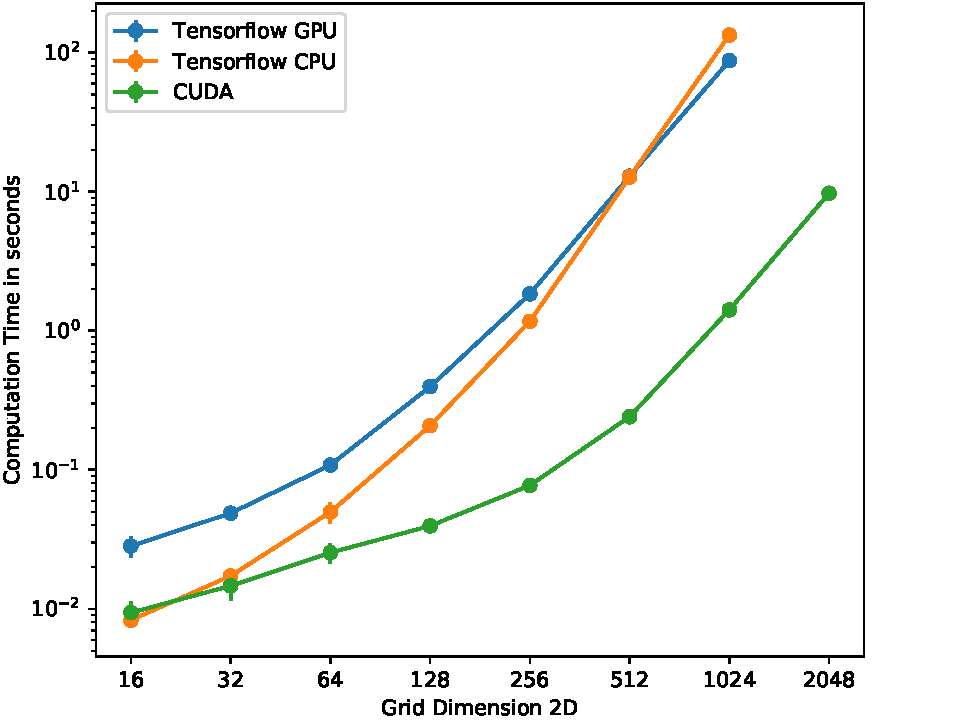
\includegraphics[height=9cm, width=14cm]{figures/performance_2d}

		\caption{Pressure Solve in 2D}
	\end{subfigure}
	\begin{subfigure}[b]{1\textwidth}
		\centering
		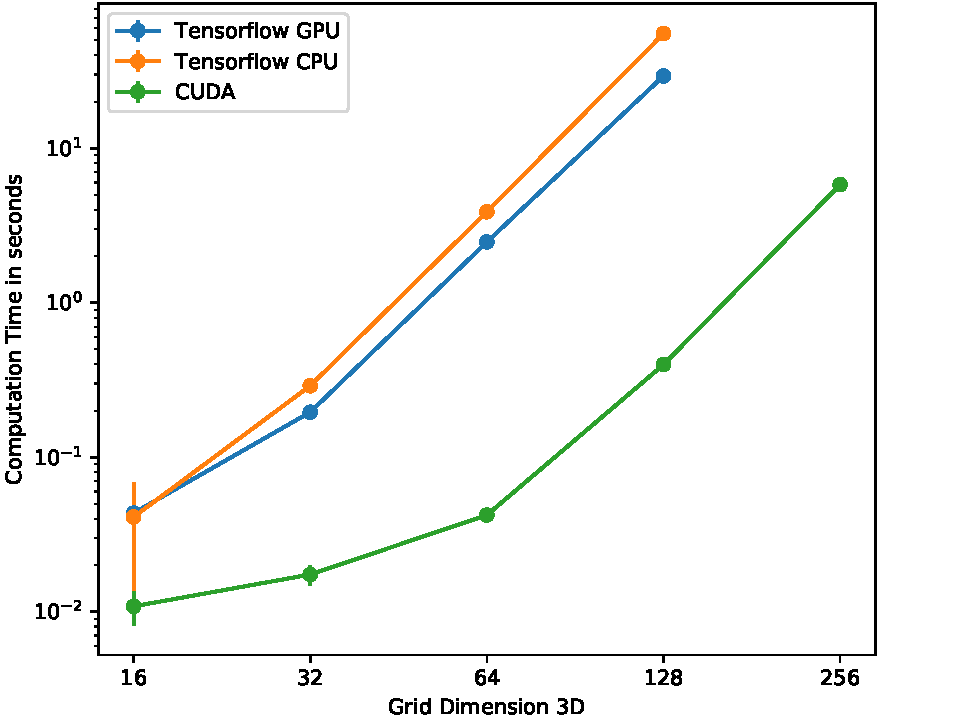
\includegraphics[height=9cm, width=14cm]{figures/performance_3d}

		\caption{Pressure Solve in 3D}
	\end{subfigure}

\caption{Execution time comparison between the three solvers.}	
\end{figure*}
